\documentclass[10pt,a4paper]{article}
\usepackage[utf8]{inputenc}
\usepackage{amsmath}
\newcommand{\RomanNumeralCaps}[1]
    {\MakeUppercase{\romannumeral #1}}
\usepackage{amsfonts}
\usepackage{amssymb}
\usepackage{float}
\usepackage{verbatim}
\usepackage{listings}
\usepackage{hyperref}
\usepackage{pbox}
\usepackage{graphicx}
%bibliography packages, bibliography files are plain text files marked .bib
%... in the same directory as the .tex file.
\usepackage[nottoc,numbib]
{tocbibind}
\usepackage{cite}
\usepackage{braket}
\usepackage{color} %red, green, blue, yellow, cyan, magenta, black, white
\definecolor{mygreen}{RGB}{28,172,0} % color values Red, Green, Blue
\definecolor{mylilas}{RGB}{170,55,241}
\usepackage{amsmath}
\usepackage{graphicx}
\graphicspath{{C:/Users/adria/Pictures/FYS3150/}}
\author{Adrian Martinsen Kleven, Simon Schrader}
\title{Project 4}

\lstset{
 	language =C++,
    frame=tb, % draw a frame at the top and bottom of the code block
    tabsize=4, % tab space width
    showstringspaces=false, % don't mark spaces in strings
    numbers=left, % display line numbers on the left
    commentstyle=\color{green}, % comment color
    keywordstyle=\color{blue}, % keyword color
    stringstyle=\color{red} % string color
}
\setlength{\columnsep}{10mm}
%\setlength{\tabcolsep}{18pt}
%\renewcommand{\arraystretch}{1.5}

\begin{document}

\part*{-Project 4 - FYS3150/FYS4150-
}
{\large By Simon Schrader (4150), Adrian Kleven (3150) - autumn 2019
}
\tableofcontents

\listoffigures
\listoftables


\clearpage

\section{Abstract}
\section{Methods}
\subsection{The Ising model in two dimensions}
The Ising model is a way of modelling macroscopic systems by simulating interactions between nearest neighbouring microscopic entities.\\The intent is to examine phase transitions in materials at finite temperatures by modelling the 2- dimensional atomic lattice as neighbouring units switching between  binary spin states. In the absence of any external magnetic field their interactions are determined by the equation
\begin{equation} \label{2d-ising energy}
E=-J\sum_{< kl >}^{N}s_ks_l 
\end{equation}
$s_k=\pm 1$. Where E is the total energy of the system and the quantity $N$ representing the total number of spins and $J$ being the coupling constant expressing the strength of the interaction between
neighboring spins \cite{Lecture_Notes_Fall_2015}.\\For a $2\times2$ lattice with binary microstates, there are 16 possible configurations:
\begin{table}[H]
\begin{tabular}{llllllllllllllll}
 $\uparrow$ $\uparrow$ &  $\uparrow$ $\uparrow$ &  $\uparrow$ $\uparrow$ &  $\uparrow$ $\uparrow$ &  $\uparrow$ $\downarrow$ &  $\uparrow$ $\downarrow$ & $\uparrow$ $\downarrow$ & $\uparrow$ $\downarrow$ \\
 $\uparrow$ $\uparrow$&  $\uparrow$ $\downarrow$ &  $\downarrow$ $\uparrow$ &  $\downarrow$ $\downarrow$ &  $\uparrow$ $\uparrow$ &  $\uparrow$ $\downarrow$ &  $\downarrow$ $\uparrow$ &  $\downarrow$ $\downarrow$
\end{tabular}
\end{table}
\begin{table}[H]
\begin{tabular}{llllllllllllllll}
 $\downarrow$ $\uparrow$ & $\downarrow$ $\uparrow$ & $\downarrow$ $\uparrow$ & $\downarrow$ $\uparrow$ & $\downarrow$ $\downarrow$ & $\downarrow$ $\downarrow$ &  $\downarrow$ $\downarrow$ & $\downarrow$ $\downarrow$ \\
 $\uparrow$ $\uparrow$ & $\uparrow$ $\downarrow$ & $\downarrow$ $\uparrow$ & $\downarrow$ $\downarrow$ & $\uparrow$ $\uparrow$ & $\uparrow$ $\downarrow$ & $\downarrow$ $\uparrow$ & $\downarrow$ $\downarrow$
\end{tabular}
\end{table}
Using periodic boundary conditions, according to equation \ref{2d-ising energy} these give instances of energy and magnetization as follows:
\begin{table}[H]
\caption[energies and magnetizations for a $2\times2$ lattice]{List of energies and magnetizations for a $2\times2$ lattice with a binary spin configuration.}
\begin{tabular}{llll}
\#Spin Up & Degeneracy & Energy & Magnetization \\
4         & 1          & -8J    & 4             \\
3         & 4          & 0      & 2             \\
2         & 4          & 0      & 0             \\
2         & 2          & 8J     & 0             \\
1         & 4          & 0      & -2            \\
0         & 1          & -8J    & -4           
\end{tabular}
\label{energies and magnetizations for a 2x2 lattice}
\end{table}
\subsection{Statistical physics}
\paragraph{The Boltzmann distribution}gives the probability of a system being in a certain configuration, and is expressed like this
\begin{equation}
P_i(\beta) = \frac{e^{-\beta E_i}}{Z}.
\end{equation}
With $\beta = \frac{1}{kT}$ being the inverse of the temperature and $k$ being the Boltzmann constant. $E_i$ is the energy of the system in the configuration $i$ and $Z$ is the partition function for the canonical ensemble
\begin{equation}
Z = \sum_{i=1}^M e^{-\beta E_i}
\end{equation}
summing over all microstates $i$. \cite{Lecture_Notes_Fall_2015}\\As an example, the partition function for the Ising model on a $2\times2$ lattice using periodic boundary conditions is
\begin{equation}
Z = \sum_{i=1}^{16} e^{-\beta E_i} = 2\left( e^{-\beta (8J)} \right) +2\left( e^{\beta (8J)} \right) +12\left( e^{0} \right)
\end{equation}
\begin{equation}
Z =  2\left( e^{-\beta (8J)} +e^{\beta (8J)} \right)+12
\end{equation}
By virtue of the partition function $Z$, the sum of the probabilities $P_i(\beta)$ for all states $i \in [1,2,\cdots,16]$ is normalized to $1$. 
\paragraph{The mean energy} of a system at a given temperature is 
\begin{equation}\label{mean energy equation}
|E| = \sum_{i=1}^{M} E_iP_i(\beta) = \frac{1}{\sum_{i=1}^M e^{-\beta E_i}} \sum_{i=1}^M E_ie^{-\beta E_i}
\end{equation}
summing over the products of the energy of a configuration with the probability of the system being in that way, then dividing by the normalization factor $Z$.\\The energy variance is calculated as
\begin{equation}\label{C_V definition equation}
\sigma_E^2 = \braket{E^2}-\braket{E}^2 = \frac{1}{\sum_{i=1}^M e^{-\beta E_i}} \sum_{i=1}^M E_i^2e^{-\beta E_i} - \left( \frac{\sum_{i=1}^M E_ie^{-\beta E_i}}{\sum_{i=1}^M e^{-\beta E_i}} \right)^2
\end{equation}
The heat capacity of the system is calculated as 
\begin{equation}
C_V = \frac{1}{kT^2} \left(  \braket{E^2}-\braket{E}^2  \right)
\end{equation}
with $k$ again, being the Boltzmann constant and $T$ being the temperature.
\paragraph{The mean magnetization} is similarly calculated:
\begin{equation} \label{Mean magnetization definition equation}
 |\mathcal{M}| = \sum_{i=1}^{M} \mathcal{M}_iP_i(\beta) = \frac{1}{\sum_{i=1}^M e^{-\beta E_i}} \sum_{i=1}^M \mathcal{M}_ie^{-\beta E_i}
\end{equation} 
with the variance
\begin{equation}
\sigma_\mathcal{M}^2 = \braket{\mathcal{M}^2}-\braket{\mathcal{M}}^2 = \frac{1}{\sum_{i=1}^M e^{-\beta E_i}} \sum_{i=1}^M \mathcal{M}_i^2e^{-\beta E_i} - \left( \frac{\sum_{i=1}^M \mathcal{M}_ie^{-\beta E_i}}{\sum_{i=1}^M e^{-\beta E_i}} \right)^2.
\end{equation}
The magnetic susceptibility then is defined as
\begin{equation}\label{Magnetic susceptibility definition equation}
\chi = \frac{1}{kT} \left( \braket{\mathcal{M}^2}-\braket{\mathcal{M}}^2 \right).
\end{equation}
\subsubsection{$2\times2$ Lattice}
From the analytical expressions, we can calculate the expectation value for the energy, the mean absolute value of the magnetic moment, the specific heat capacity and the magnetic susceptibility of the $2\times 2$ lattice.\\Starting with the energy terms, $|E|$ and $\braket{E^2}$ are calculated first using equation \ref{mean energy equation}.
\begin{equation*}
|E|(\beta) = \frac{1}{\sum_{i=1}^{16} e^{-\beta E_i}} \sum_{i=1}^{16} E_ie^{-\beta E_i}
\end{equation*}
\begin{equation}
|E|(\beta) = \frac{8J\left( e^{-\beta (8J)} -e^{\beta (8J)} \right)}{ e^{-\beta (8J)} +e^{\beta (8J)} +6}.
\end{equation}
Inserting $E_i^2$ for $E_i$ into equation \ref{mean energy equation} gives
\begin{equation*}
\braket{E^2}(\beta) = \frac{\sum_{i=1}^{16} E_i^2e^{-\beta E_i}}{2\left( e^{-\beta (8J)} +e^{\beta (8J)} \right)+12}
\end{equation*}
\begin{equation}
\braket{E^2}(\beta) = \frac{32J^2\left( e^{-\beta (8J)} +e^{\beta (8J)} \right)}{\left( e^{-\beta (8J)} +e^{\beta (8J)} \right)+6}.
\end{equation}
From equation \ref{C_V definition equation} we then get
\begin{equation}
C_V = \frac{1}{kT^2}\left( \frac{32J^2\left( e^{-\beta (8J)} +e^{\beta (8J)} \right)}{\left( e^{-\beta (8J)} +e^{\beta (8J)} \right)+6}  - \left( \frac{8J\left( e^{-\beta (8J)} -e^{\beta (8J)} \right)}{ e^{-\beta (8J)} +e^{\beta (8J)} +6} \right)^2 \right).
\end{equation}

Next is calculating the mean absolute value of the magnetic moment. In doing this, the magnetization is treated the same if it is of the same magnitude but in the opposite direction. Magnetization from this point forward will mean exactly this. That means the instances of magnetization are as in table \ref{energies and magnetizations for a 2x2 lattice}, but with negative instances of magnetization counting towards their respective absolute value. Using equation \ref{Mean magnetization definition equation},
\begin{equation*}
|\mathcal{M}| = \frac{\left( 2\left( 4e^{\beta (8J)} \right) +8\left( 2\cdot1 \right)\right)}{2\left( e^{-\beta (8J)} +e^{\beta (8J)} \right)+12} = \frac{4\left(  e^{\beta (8J)}  +2\right)}{ e^{-\beta (8J)} +e^{\beta (8J)}+6}.
\end{equation*}
For calculating $\braket{\mathcal{M}^2}$, $\mathcal{M}^2$ is inserted for $\mathcal{M}$ in equation \ref{Mean magnetization definition equation}.
\begin{equation*}
\braket{\mathcal{M}^2}(\beta) = \frac{\sum_{i=1}^{16} \mathcal{M}_i^2e^{-\beta E_i}}{2\left( e^{-\beta (8J)} +e^{\beta (8J)} \right)+12}  = \frac{2\left( 16e^{\beta (8J)} \right) +8\left( 4\cdot1 \right)}{2\left( e^{-\beta (8J)} +e^{\beta (8J)} \right)+12}  
\end{equation*}
\begin{equation}
\braket{\mathcal{M}^2}(\beta) = \frac{ 16\left( e^{\beta (8J)}  +1 \right)}{\left( e^{-\beta (8J)} +e^{\beta (8J)} \right)+6}.
\end{equation}
The magnetic susceptibility can then be calculated using equation \ref{Magnetic susceptibility definition equation}.
\begin{equation}
\chi = \frac{1}{kt}\left( \frac{ 16\left( e^{\beta (8J)}  +1 \right)}{\left( e^{-\beta (8J)} +e^{\beta (8J)} \right)+6} - \left( \frac{4\left(  e^{\beta (8J)}  +2\right)}{ e^{-\beta (8J)} +e^{\beta (8J)}+6} \right)^2 \right)
\end{equation}
These equations will later be useful for benchmarking our program by comparing computed values to the analytical expressions.
\subsubsection{Phase transition}
Phase transitions are sudden changes in properties relating to a change in external parameters such as temperature. The temperature at which such a transition takes place is called the critical temperature. The Ising model in two dimensions with no external magnetic field undergoes a second order phase transition \cite{Lecture_Notes_Fall_2015}. This phase transition is characterized by spontaneous magnetization occurring below the critical temperature $T_C$ and an average magnetization of zero above $T_C$\cite{Lecture_Notes_Fall_2015}.
\paragraph{The correlation length $\xi$}is a function of temperature and it describes the degree with which two spins separated by some distance are correlated. When temperatures are much greater than the critical temperature, $\xi$ is expected to be of the order of the lattice. However, at temperatures close to the critical temperature, the correlation length for a second order phase transition will come to span the length of the entire system \cite{Problem_set_4}, meaning every spin is correlated with every other spin. The behaviour of $\xi$ for $T$ close to $T_C$ is characterized by
\begin{equation}
\xi(T)\sim \left| T_C-T \right|^{-\nu}.
\end{equation}

\subsubsection{Extracting the critical temperature}
\subsection{The Metropolis algorithm}

\subsection{Periodic boundary conditions}
Because it is not computationally possible to simulate a system in the magnitude of real matter (which is close to Avogadro's number), a simulated system has a much higher surface-per-volume ratio \footnote{In the case of a two-dimensional system, it is technically a border-per-surface ratio.} than a real system. This needs to be taken into consideration, because otherwise, simulation results would ignore a large part of interactions existing in larger systems. One way to tackle this issue, is to employ periodic boundary conditions. The idea is that the particles on the system's borders interact with each other. That is, in a lattice of size $n\times n$, the particles in the $n$\textsuperscript{th} row or column interact with the particles in the first row or column, as if they were in the  $(n+1)$\textsuperscript{th} row or column. The advantage of this is that there are no surface particles, thus simulating an infinity large system, resembling reality closer than a very small system. The disadvantage is that particles are correlated in an unnatural way. Especially in smaller systems, this will lead to particles interacting with their own "mirror image", where a particle's spin conformation might affect the surrounding in a way that the particle itself will be affected by its own spin.
All simulations were done using periodic boundary conditions.
\subsection{Computational implementation}

\subsubsection{Units}
In this simulation, we simply assume the individual spins to be unitless. Thus, the magnetisation is unitless as well.
The energy is scaled as the unitless $\tilde{E}=E/J$, the Temperature is scaled as  $\tilde{T}=\frac{k}{J}T$. This ensures that the exponent is unitless.
Then, the Heat Capacity $C_V$, defined as $\frac{\sigma_E^2}{kT^2}$, is given as $\frac{J^2\sigma^2_{\tilde{E}}}{k\frac{J^2}{K^2} \tilde{T}^2}=\frac{\sigma^2_{\tilde{E}}}{\tilde{T}^2}k$, that is, it is reported as a multiple of k. 
Similarly, The susceptibility $\chi$, defined as $\frac{\sigma_{|M|}^2}{kT}$, has units $\frac{1}{J}$. For simplicity, tilde-symbols are dropped in later discussions, and when stating the temperature in the text, it's unit is omitted.
\subsubsection{Analytical solution}
The implementation of the analytical solution is rather straightforward. For each spin, a for-loop is implemented (within a previous for-loop), that loops over each permitted state (1 and -1). That system's magnetization and energy are then calculated using the formulas stated above and stored in an array. From the energies, the probabilities and the partition function can be calculated for a given temperature. One can than calculate $E[E],E[E^2],E[M]$, and $E[M^2]$ and thus find the system's susceptibility and heat capacity. However, this scales as O($2^N$) because there are  $2^N$ microstates where N is the amount of spins, this becomes a very expensive calculation even for latices where e.g. the lattice size L=5 (N=25), and is clearly not doable for large lattices. Here, only the case L=2 was implemented.
\subsubsection{Efficient formulas}
The system's total energy upon switching one spin state is changed by any of $\Delta E \in \{-8J,-4J,0,4J,8J\}$ because 
$$\Delta E=E_2-E_1=J\sum_{<kl>}^Ns_k^1s_l^1-J\sum_{<kl>}^Ns_k^2s_l^2$$
Because only one individual spin $s_l$ is changed, that can be rewritten as 
$$\Delta E=-J\sum_{<kl>}^Ns_k(s_l^2-s_l^1)$$
Then, because $s_l^1-s_l^2$ is either 2 or -2, depending on the value of $s_l^1$, the final change in energy can be written as 
$$\Delta E=2Js_l^1\sum_{<kl>}^Ns_k$$
As the change in magnetisation only depends on the particle $s_l$, it is either -2 (1 to -1) or 2 (-1 to 1), so the change in the magnetisation is given as 
$$\Delta M=-2s_l^1=2s_l^2$$
The relative difference in probability between two spin states, which is the actual selection rule for the Metropolis algorithm, is then given by  
$$\frac{exp(-E_2/T)}{exp(-E_1/T)}=exp(-\Delta E/T)$$
This can be precomputed for each individual $\Delta E$ for a given temperature and stored in an array to be reused, which saves computational time. 
\subsubsection{Simulating the system}
The lattice was implemented as a two-dimensional integer matrix with values -1 or 1, representing the spin states. The initial matrix is either randomized or has all spins pointing in the same direction (see Results-part). 
Then, the initial energy and magnetisation can be calculated using the formulas above.
The Metropolis algorithm was then implemented the following way after the system has been set up:\\
N times, where $N=L^2$ and L is the lattice size, a suggested spin to flip is suggested. Then the change in energy and $exp(-\Delta E/T)$ are calculated.If $exp(-\Delta E/T)$ is larger than a randomly distributed number r \footnote{The Mersenne-Twister RnG is used to create this number}, the move is accepted, otherwise the loop over N is continued. If the move is accepted, the system's magnetisation and the energy are updated. After the loop is finished, the expectation values for $E$, $E^2$, $M$, $M^2$ are updated. The loop is then repeated for the desired amount of simulation steps. Finally, the final expectation values for $E$, $E^2$, $M$, $M^2$, $C_V$ and $\chi$ are calculated.\\
In order to do this for different lattice sizes L and different temperatures, this whole procedure was implemented in two more loops, one looping over the temperatures and one looping over the lattice sizes.
\subsubsection{Parallelization}
In order to increase computational performance, the time-consuming calculations were parallelized using openMPI. The computational implementation has 3 nested loops: One loop iterating over each temperature, one loop iterating over the different lattice sizes, and one loop implementing the actual Metropolis algorithm\footnote{Technically, two more nested loops were implemented within the Metropolis algorithm, but they could equally well be implemented as a part Metropolis loop itself.}. Because the Metropolis algorithm explicitly depends on the earlier state, and because simulating smaller lattice sizes requires less time, the temperature loop was parallelized. This was done by giving each thread a different start temperature (with a spacing of the given temperature step between each thread), and giving each thread a "new" temperature step, which is the original temperature step times the amount of threads. The advantage of this implementation is that it is fairly simple to implement, and from the results, it is easy to inspect that it was implemented correctly. The disadvantage is that it does not give ideal run time if the total amount of time steps is not divisible by the amount of threads, leading to one or several threads finishing earlier than the rest. \\
In order to improve the run time even more, we also tested several compiler flags, both for the parallelized and the non-parallelized version, in order to see how to achieve the best possible time.
\subsubsection{Unit testing}
We tested that the system was sat up correctly and that the resulting numbers and calculations are correct  by comparing the simulation for a $2\times2$-lattice with the analytical solution at different temperatures. The requirement is that, after $10^6$ simulations, the standard error compared to the analytical solution is required to be less than than 1\%.
\subsubsection{Calculating the critical temperature}
The critical temperature can, as described earlier, be extracted using the formula 
$$T_C(L)-T_C(L=\infty)=a\cdot L^{-1/v}$$
where L is the lattice size and $T_C(L)$ is the critical temperature in the non-infinite system. Here, v=1. This can be reformulated as 
$$T_C(L)=a\cdot L^{-1}+T_C(L=\infty)$$
As $T_C(L)$ will be known from the simulations, and L is a preset factor, there are only two unknown constants: $a$ and $T_C(L=\infty)$. Those can then be found using linear regression, and the insecurity in the critical temperature at $L=\infty$ can be estimated to be the standard deviation of the points from the straight line.
\section{Results}
\subsection{Reaching the equilibrium state}
When setting up the initial lattice, we tested whether it is better to start with a random distribution of spins, or start with all spins pointing in the same direction. A simple way to do that is to visualize the system's average energy, average magnetisation and percentage of accepted configurations for a given amount of steps, as a function of the total amount of steps. We did that for two temperatures, T=1.0 and T=2.4, for lattices sized $20\times20$ and $100\times 100$, and plotted the results. This can be seen in figure \ref{Average energy, average absolute magnetisation and accepted spins at T1.0} and figure \ref{Average energy, average absolute magnetisation and accepted spins at T2.4}.
\begin{figure}[H]
%\centering
    \includegraphics[width=\textwidth]{configurations_200_size_1,0_temp.pdf}
\caption[Average energy, average absolute magnetisation \& accepted spins at T=1.0]{The system's average energy, its absolute magnetisation and the percentage of accepted spins as a function of the simulation step for a $20\times20$ lattice at temperature T=1.0. Up is all spins pointing up initially, random is randomized spin distribution.}\label{Average energy, average absolute magnetisation and accepted spins at T1.0}
\end{figure}
\begin{figure}[H]
\includegraphics[width=\textwidth]{configurations_200_size_2,4_temp.pdf}
%\centering
\caption[Average energy, average absolute magnetisation \& accepted spins at T=2.4]{The system's average energy, its absolute magnetisation and the percentage of accepted spins as a function of the simulation step for a 20x20 lattice at temperature T=2.4.Up is all spins pointing up initially, random is randomized spin distribution.}\label{Average energy, average absolute magnetisation and accepted spins at T2.4}
\end{figure}
One can clearly see that the magnetisation, the energy and the amount of accepted configurations behave similarly in the sense that they all tend to equilibrate after approximately the same amount of steps.
The results produced using a $100\times100$ lattice gave similar results, indicating that these results can be used for any lattice size between 20 and 100. One can see clearly that the state with all spins pointing up is equilibrated after around 20,000 steps for both temperatures. At T=2.4, both the randomized system and the system with all spins pointing up seem to take the same amount of steps to equilibrate. However, for T=1.0, the randomized spin distribution seems to require more steps.\footnote{This might however be an illusion, as the plots visualize the \textit{total} averages. Very large discrepancies in the first steps might alter the averages long-term, even though the system already is in equilibrium.}\\
For these reasons, the larger simulations were sat up using an initial systems where all spins point up, and the first 20,000 steps were discarded. 
After the equilibrium state has been reached, one can start to sample in order to calculate several physical units of the system. 
Another interesting observation is that many more states are accepted at the higher temperature - while only slightly more than 0.05\% states are accepted at T=1.0, over 25\% are accepted at T=2.4. This is expected - The exponent $\frac{-\Delta E}{T}$, that is, the sampling rule, for positive values of $\Delta E$, is much larger for larger values of T, thus much more moves are accepted. This fits well with the discussion of the energy distribution described below - as moves are accepted, there is much more fluctuation among the different states, which leads to a broader distribution of energies. 
\subsection{Time benefit from Parallelization and compile flags}
Parallelization gave a substantial time benefit, however, different compilation flags barely changed the program's run time. The program was run on a computer with a CPU with 4 cores, and 8GB RAM. Table XXX shows the time usage (single runs) achieved with different compilation flags, with- and without parallelization. A rather short timing experiment was conducted, and it is run over 4 temperatures in order to achieve the ideal speedup from parallelization.
\begin{table}[H]
\centering
\caption[Time usage parallel/non-parallel, compilation flags]{Time consumption of a simulation using $4\cdot10^4$ simulation steps for 4 different temperatures (T=2.0,2.1,2.2,2.3) and 4 matrix sizes (L=40,60,80,100) with different compiler flags. All results were averaged over 4 runs}
\centering
\begin{tabular}{|r|r|r|}
\hline
Compiler flag & Time (parallel) [s] & Time (non-parallel) [s] \\ \hline
None             & 153                 & 507                     \\ \hline
-O2              & 149                 & 507                     \\ \hline
-O3              & 150                 & 496                     \\ \hline
-Ofast           & 137                 & 503                     \\ \hline
\end{tabular}
\end{table}
The big improvement in timing clearly comes from parallelization: The time usage is more than 3 times higher for the non-parallelized code. However, it is not 4 times higher for any of the chosen compiler flags - this might be due to imperfect implementation of parallelized code, among them the fact that the program, in the end, only runs with one active thread that is not finished yet. The compiler flags have a very minute effect on the run time of the non-parallelized code, speeding it up by less than 3 percent, while only the -Ofast-flag leads to appreciable improvement of ca. 10 percent in the run time of the parallelized code. However, these numbers fluctuated wildly, as can be seen in the file "time.csv" on GitHub. Thus, it is quite possible that there really is no speed-up on the long run. The larger simulations were run using the -Ofast- flag nevertheless.

\subsection{Results achieved using 2x2 lattice}
Using a 2x2 lattice, the same results where achieved as for the analytical solution, which indicates that the algorithm was implemented correctly and gives reasonable results. The actual results are not interesting and not presented here. Because these simulations are comparatively fast to run, it is feasible to compute the relative error found in these calculations and use them to get a very general idea on error estimation for the calculations where no analytical solution can be computed.
Using $10^6$ simulation steps, the relative error could be reduced to less than one percent for all physical quantities for temperatures between 2.0 and 3.0. However, there were huge fluctuations in the maximum relative error, and the maximum relative error was always found in the heat capacity. Example data can be found in the appendix.
\subsection{Energy distribution in a 20x20 lattice}
As the temperature is increased, the system's average energy increases as well. The energies' probability distribution is changed as well. These probability distributions for a T=1.0 and T=2.4 in a 20x20 lattice are shown in figure \ref{Energy probability distributions in a 20x20 lattice at T1.0  T2.4}.
\begin{figure}[H]
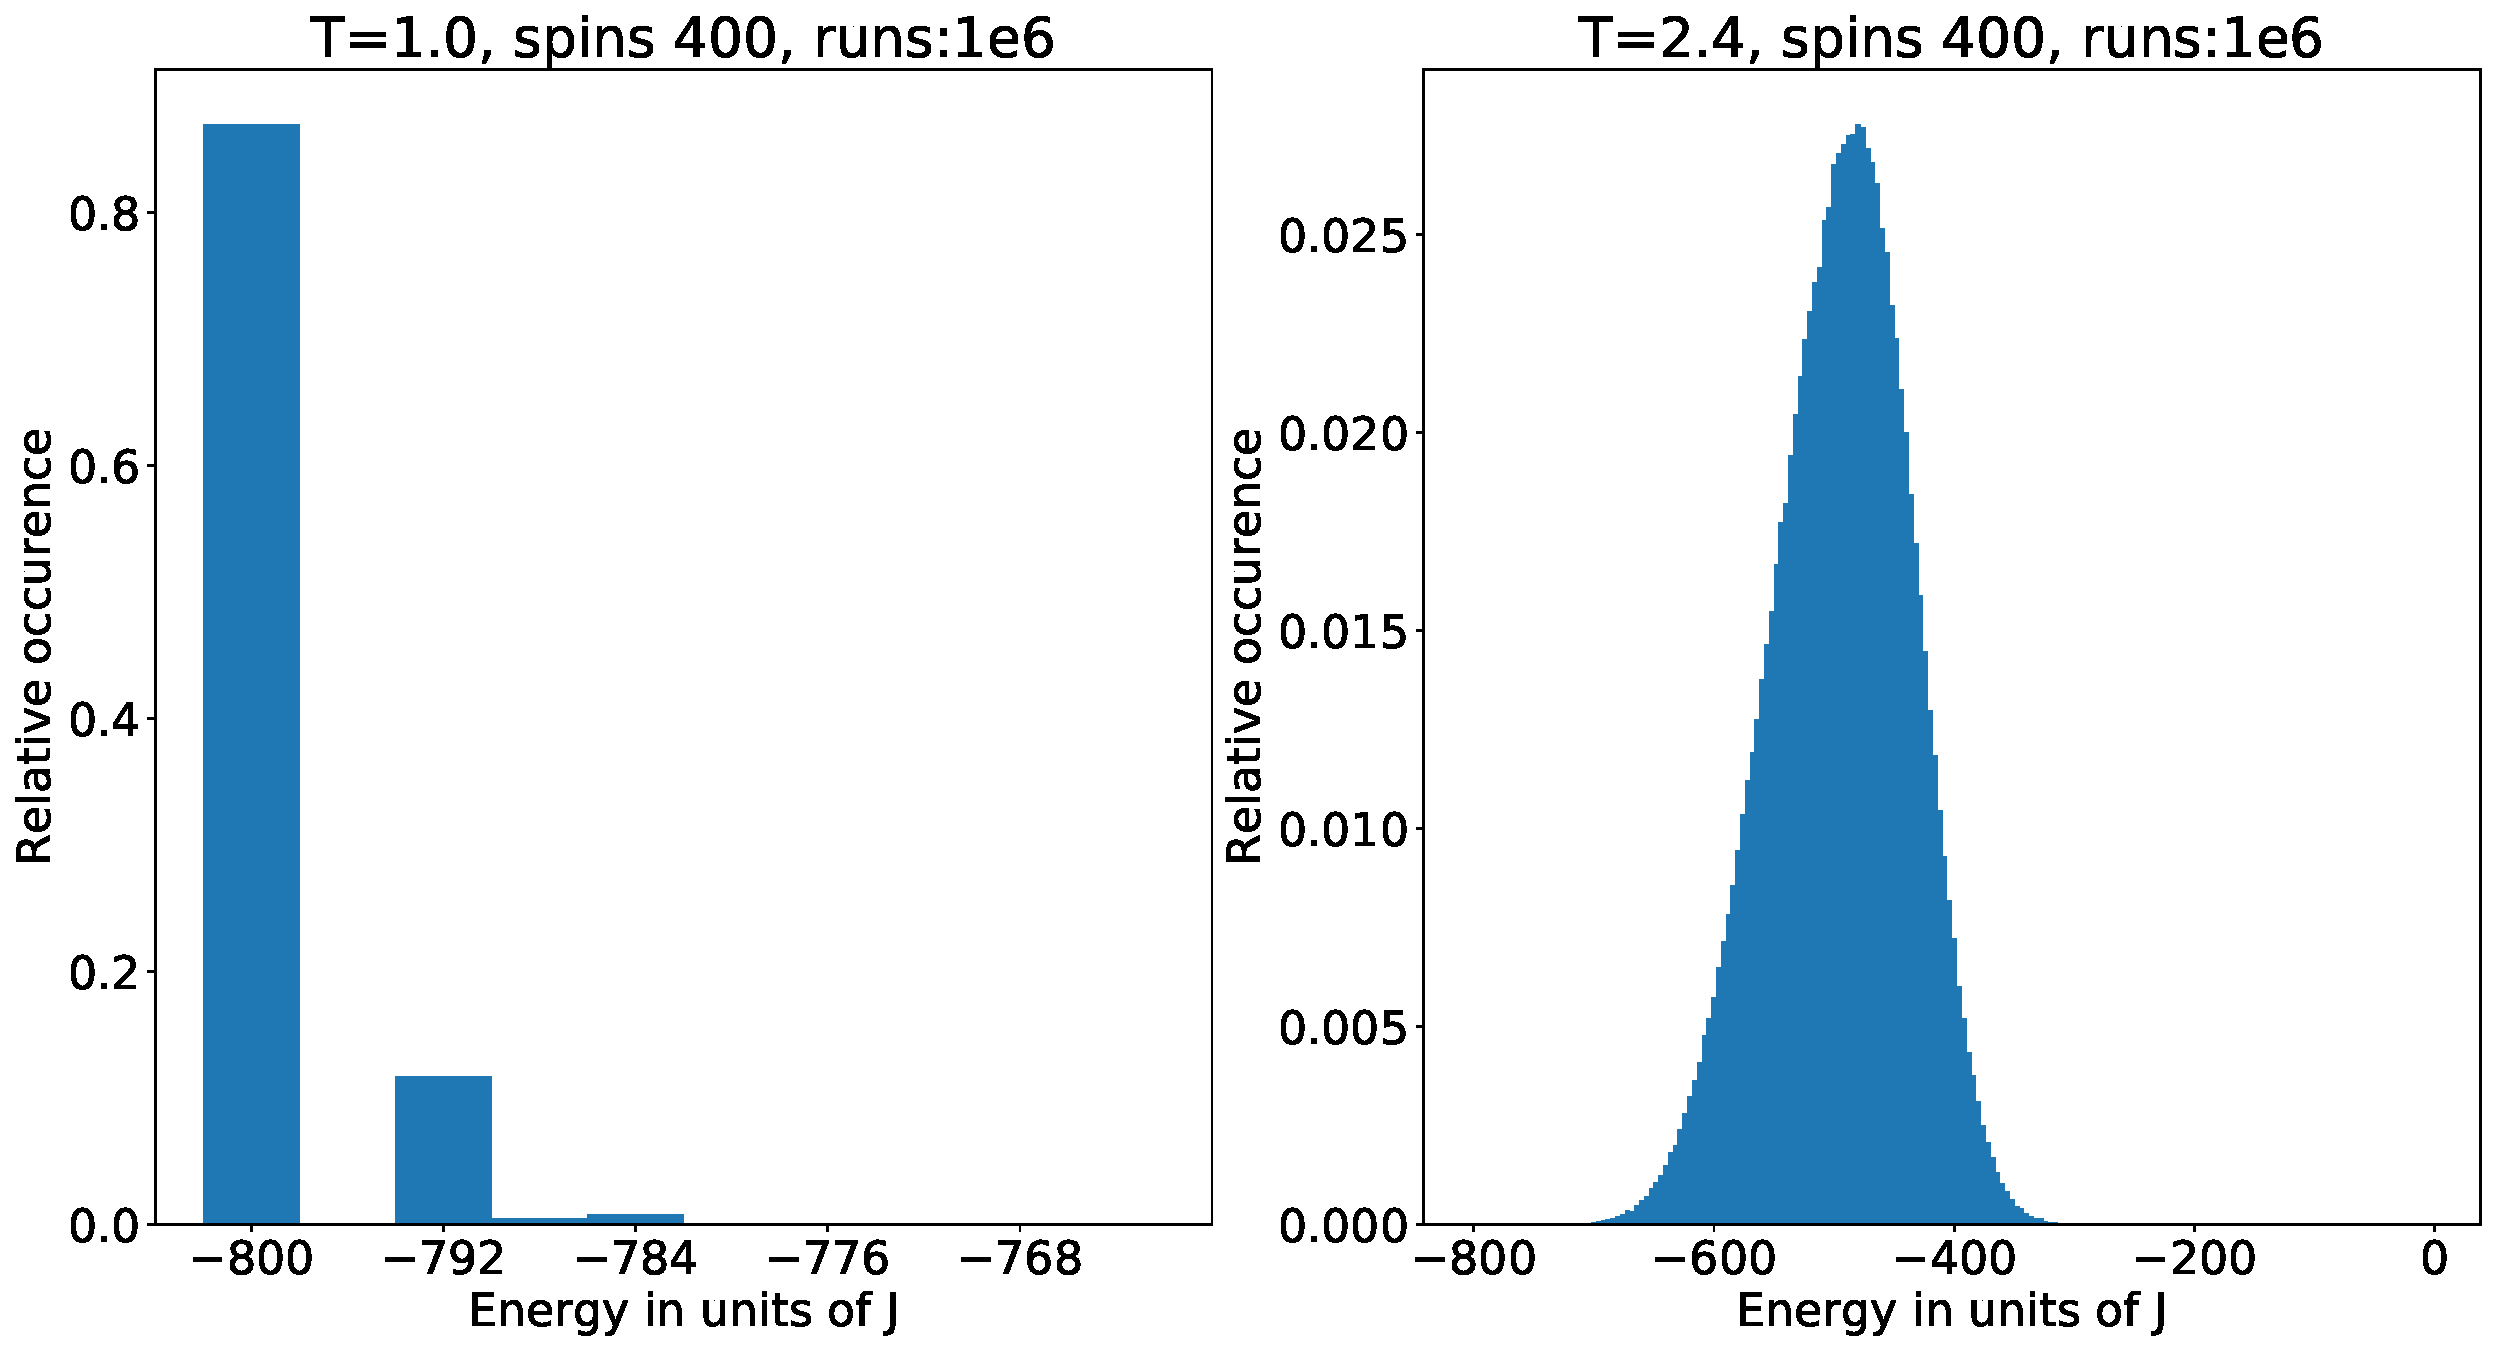
\includegraphics[width=\textwidth]{Dist.pdf}
%\centering
\caption[Energy probability distributions in a 20x20 lattice at T=1.0 \& T=2.4]{Distribution of energies in a $20\times20$ lattice at T=1.0 and T=2.4 with $10^6$ simulation steps.}\label{Energy probability distributions in a 20x20 lattice at T1.0  T2.4}
\end{figure}
This data fits well with the calculated standard deviations. At T=1.0, the standard deviation in energy is $\sigma_E\approx3.05J$ around the average value $E=-798.8J$, at T=2.4, the standard deviation in energy is $\sigma_E\approx57.1J$ around the average value $E=-495.0J$. At the higher temperature, the energies are distributed over a much broader range, and far more individual energies have a nonzero distribution. This data fits also very well with Figure \ref{Average energy, average absolute magnetisation and accepted spins at T1.0} and Figure \ref{Average energy, average absolute magnetisation and accepted spins at T2.4} - far more suggested configurations are accepted at T=2.4, which clearly increases the fluctuation in energy and thus the standard deviation, compared to the low-temperature state. From this, we can also see that the system at T=2.4 has a much higher heat capacity, which is closely related to the standard deviation. This fits with the calculated data, where the individual particle's heat capacity is given as $C_V$=1.4 for T=2.4 and $C_V$=0.023 for T=1.0. 
\subsection{Behaviour of the system close to the critical temperature}
Thanks to calculations done by Lars Onsager \cite{onsager1944two}, we know that the Ising model has an analytical critical temperature of $T_C\approx2.269$, where a phase transition should occur. This behaviour is also expected to show up in a simulation, and a large enough lattice with enough simulation steps should give a result close to the analytical solution.\\We ran a simulation of lattices of sizes L $\forall L \in \{40,60,80,100\}$ for temperatures ranging from 2.0 to 2.35 with a step length of $\Delta T=0.05$ in order to get an overview over the systems' behaviour in the vicinity of the critical temperature. These simulations were run with $10^6-20,000$ simulation steps. The results are shown in figure \ref{for T between 2.0 and 2.35}. Note that the susceptibility $\chi$ is calculated from the absolute value of the magnetization. 
\begin{figure}[H]
%\centering
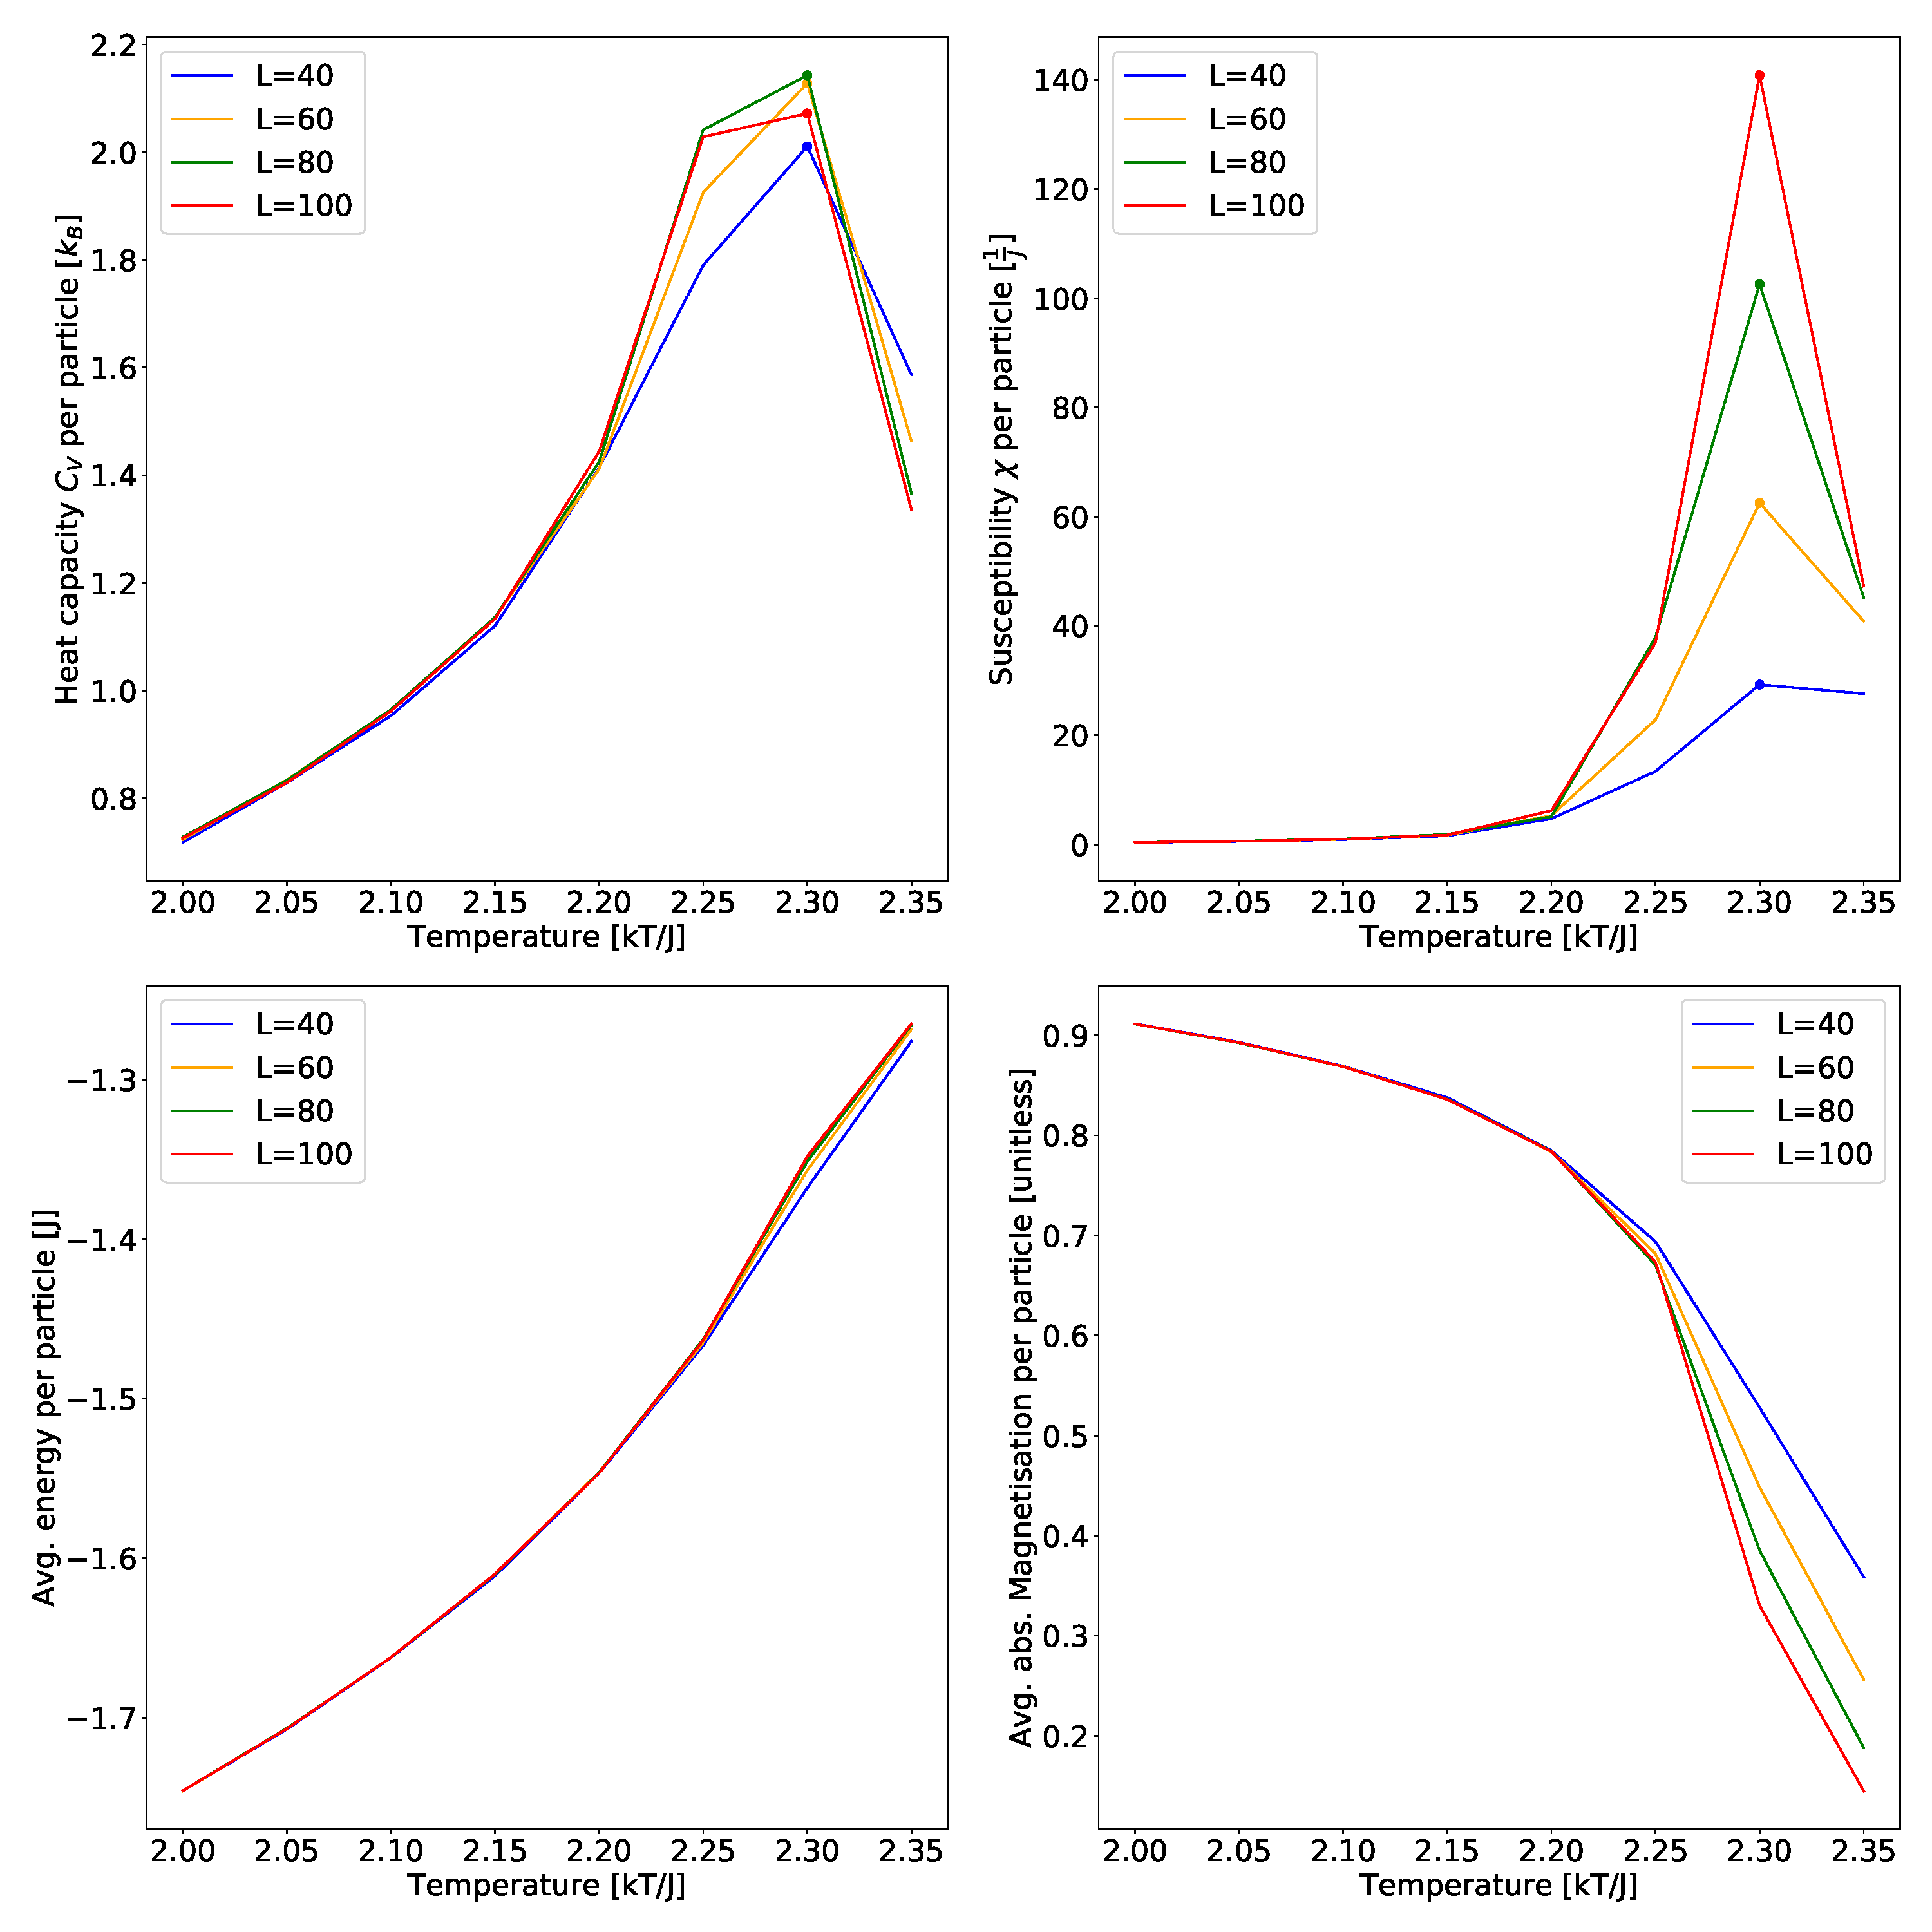
\includegraphics[width=\textwidth]{results_calculations_general.pdf}
\caption[$C_V,\chi,E, |M|$ for T between 2.0 and 2.35]{$C_V,\chi,E$ and $|M|$ as functions of T for  L $ \in \{40,60,80,100\}$ for T between 2.0 and 2.35 with a step length of $\Delta T=0.05$. For each temperature, $10^6-20,000$ simulation steps were carried out. Maximum value is marked for $\chi,C_V$.}\label{for T between 2.0 and 2.35}
\end{figure}
From these graphs, a whole lot of information can be extracted. All four systems behave almost identically for temperatures below 2.2 (the curves overlap), however, at temperatures close to the analytical critical temperature, the curves separate. This is in accordance with formula XXX, which states that the divergence from the real critical temperature is a function of lattice size. This is especially interesting to observe for the absolute magnetisation, where the value at T=2.35 is getting smaller and smaller as the lattice size increases.\\
Another observation is that the simulated critical temperature gets closer and closer to the real critical temperature as the lattice size increases, which also is in accordance with formula XXX. This can be observed by the "steepness" in the curves of the heat capacity: For L=40, it is much higher at T=2.30 than at T=2.25, indicating that it is much closer to 2.30, while at L=100, the values for T=2.30 and T=2.25 are almost identical. The steep drop from T=2.30 to T=2.35 indicates that it is closer to T=2.25 than to T=2.35 for all four systems.\\
Finally, one can observe how the maximum values for $\chi$ and $C_V$ increase with the systems size, indicating that they reach infinity as L approaches infinity.\\\\
In order to get a better estimate on the simulated systems' critical temperature, another simulation was carried out, with a more narrow range for the temperatures, and more simulation steps. A simulation with T between 2.20 and 2.35 and $3.48\cdot10^6$ simulations for 8 temperatures with equal spacing is shown in figure \ref{for T between 2.20 and 2.35} in the appendix. From there, one can see that the critical temperature for both the susceptibility and the heat capacity lies between T=2.265 and T=2.315 (but for $\chi$ when L=40). We ran a last simulation consisting of only this temperature interval, with XXX simulation steps. The results can be found in figure \ref{for T between 2.265 and 2.315} in the appendix.
\subsection{Calculating the critical temperature}
The critical temperature can be calculated using the procedure above. Doing this, we find that $T_C(L=\infty)\approx$. Even though the method gives accurate results in theory, because $T_C(L)$ is only an approximation (it might be at slightly higher or slightly lower temperatures; and more simulation steps would increase the accuracy), the found critical temperature is not perfectly identical to the analytical result. Nevertheless, it is quite close to it (XXX and the real value is within the standard deviation XXX).
\section{Conclusion}
Using simulations, it is possible to learn a lot about physical systems. The Metropolis algorithm has shown to be quite reliable, and the simulated result is quite close to the analytical result. The Ising model is quite primitive in the sense that several quantities showing up in real systems are ignored, such as length or charge, or that particles only interact with their nearest neighbours, or that matter in fact is 3- dimensional. But it still has many important physical attributes that one can calculate. In more sensitive simulations, this is something to be taken into consideration, but it exceeds the frame of this article. Using gradient-based techniques, it might be possible to approximate a simulated system's critical temperature without having to do simulations for each temperature where one might suspect the critical temperature to be. 
We did not employ methods such as reshuffling (Bootstrap, for example) to get better guesses on the critical temperature, and we didn't include aspects such as covariance that might be caused by, for example, the random number generator. This could be done in future articles.
\section{Critique}

\section{Appendix}
\subsection{Figures}
\begin{figure}[H]
%\centering
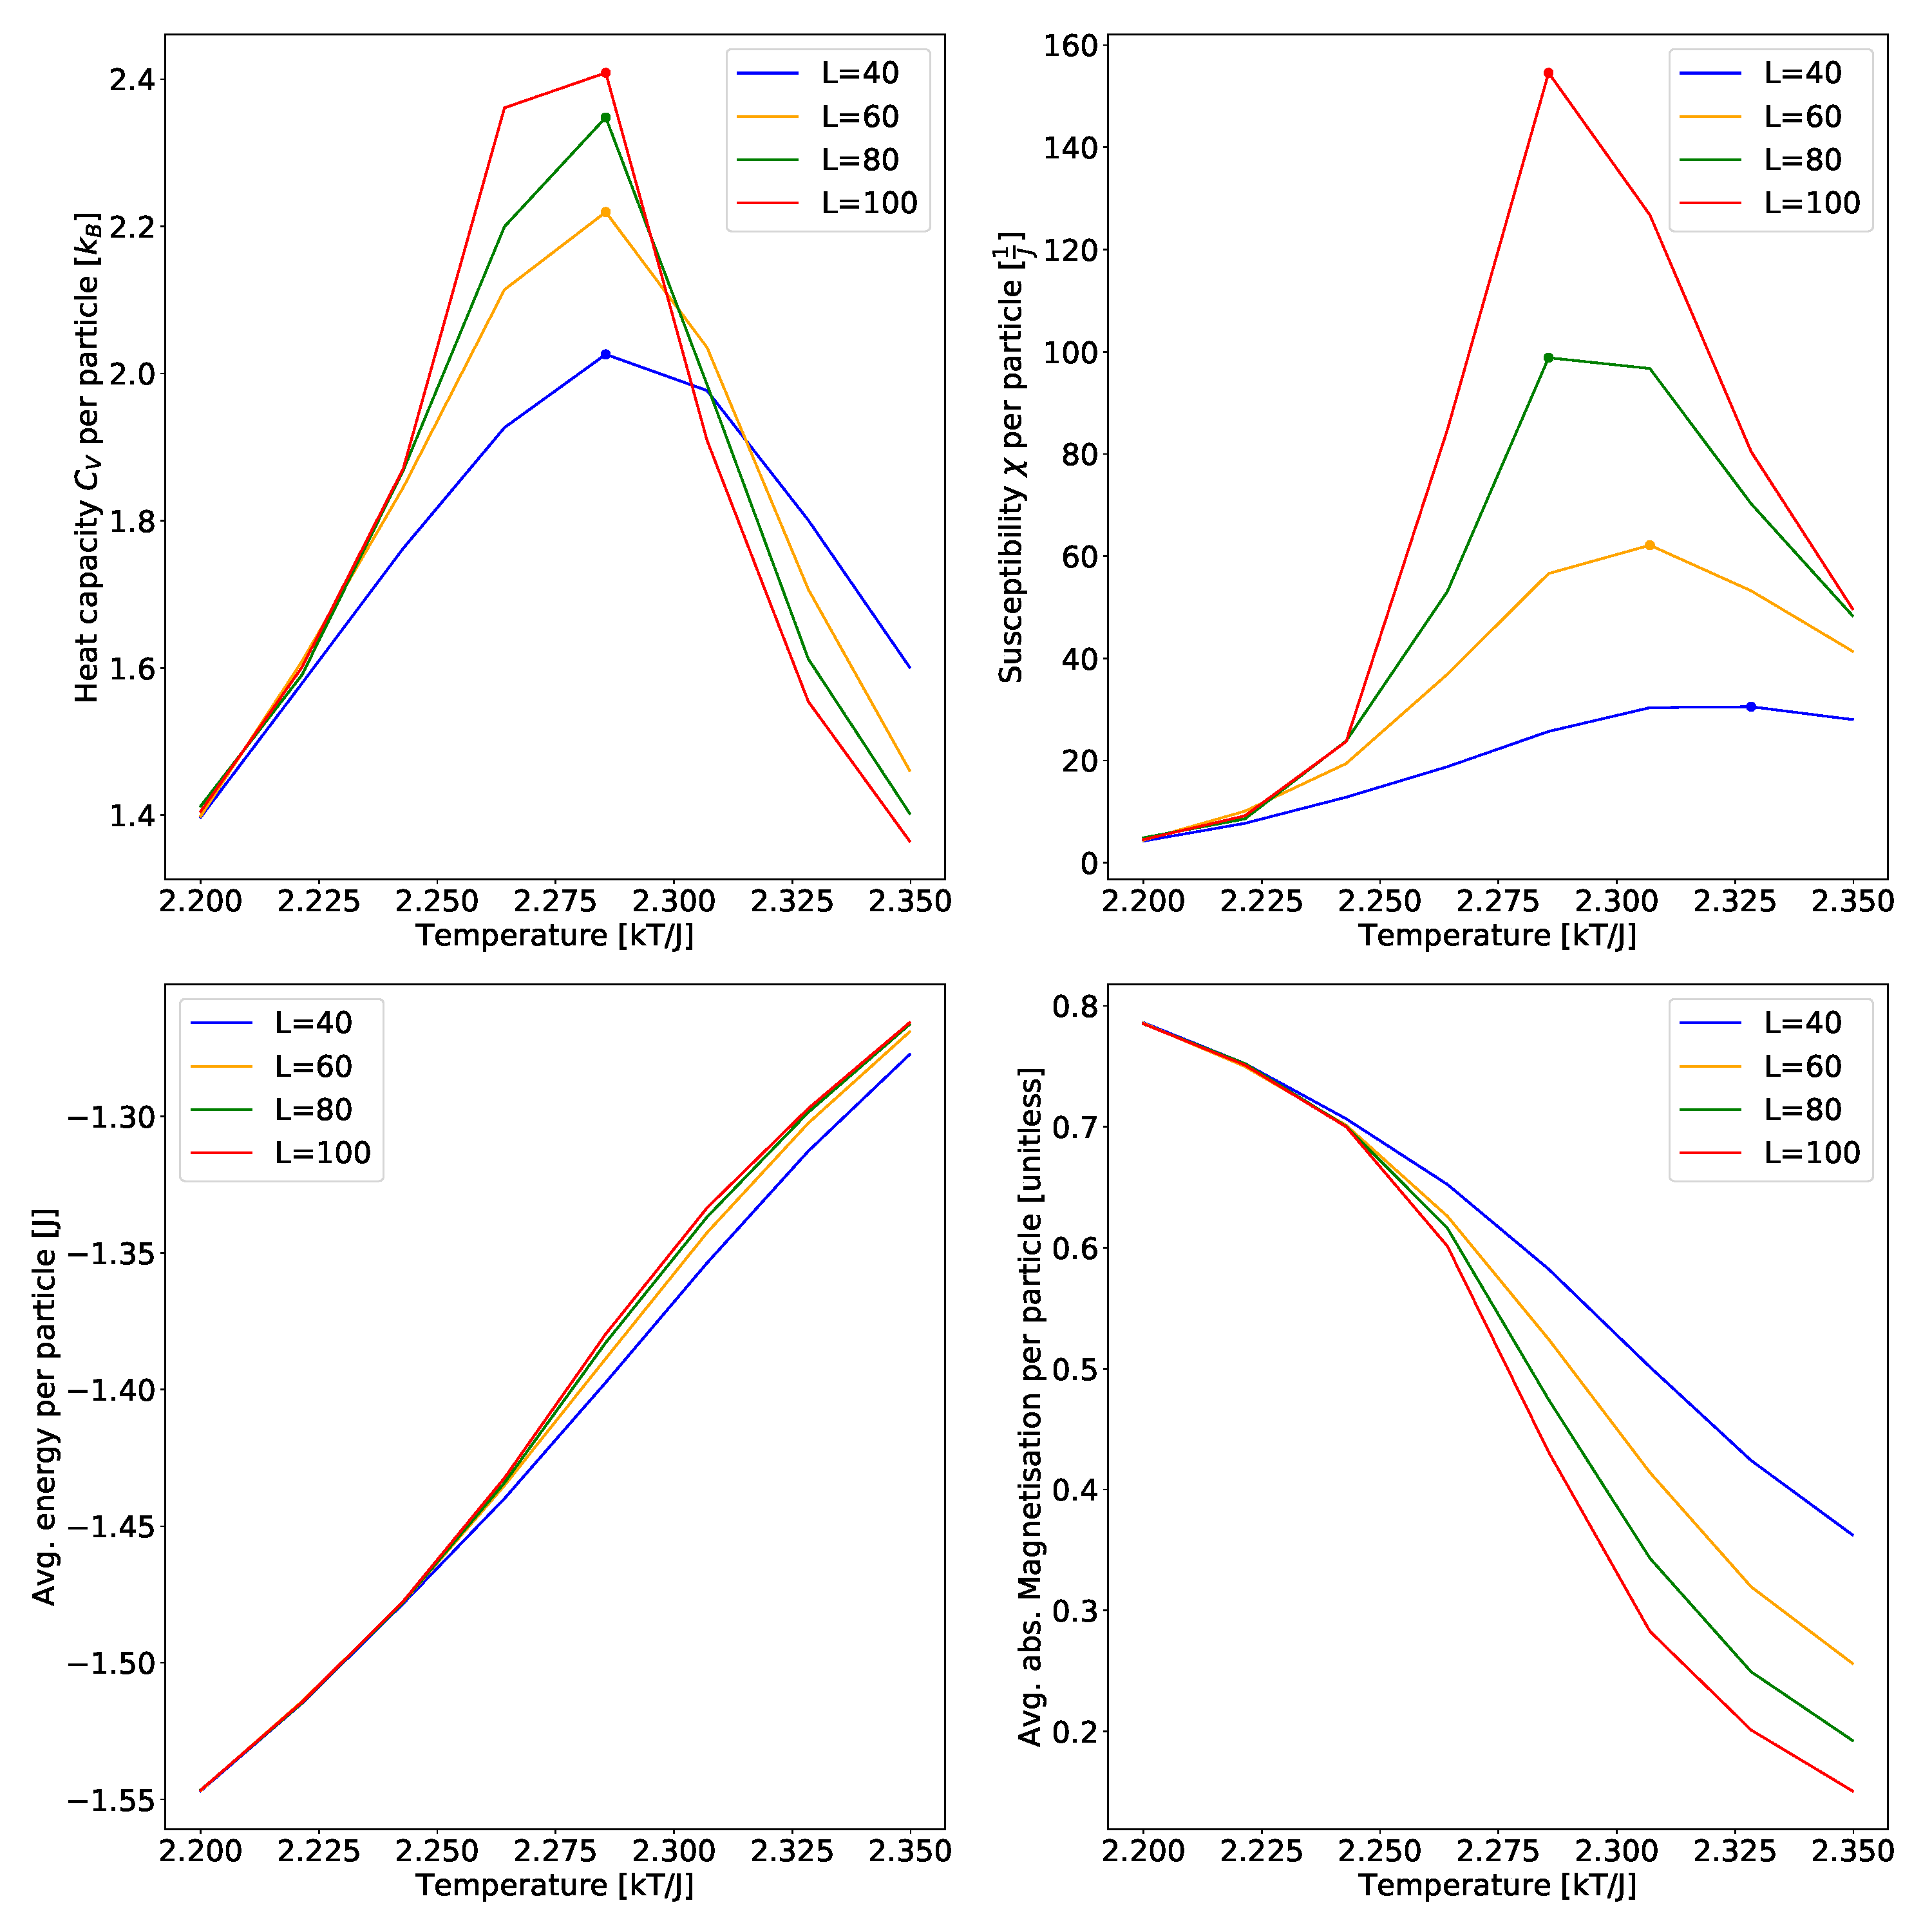
\includegraphics[width=\textwidth]{results_calculations_more_accurate.pdf}
\caption[$C_V,\chi,E, |M|$ for T between 2.20 and 2.35]{$C_V,\chi,E$ and $|M|$ as functions of T for  L $ \in \{40,60,80,100\}$ for T between 2.20 and 2.35 with a step length of $\Delta T=0.0214$. For each temperature, $3.48\cdot10^6$ simulation steps were carried out. Maximum value is marked for $\chi,C_V$.}\label{for T between 2.20 and 2.35}
\end{figure}

\begin{figure}[H]
%\centering
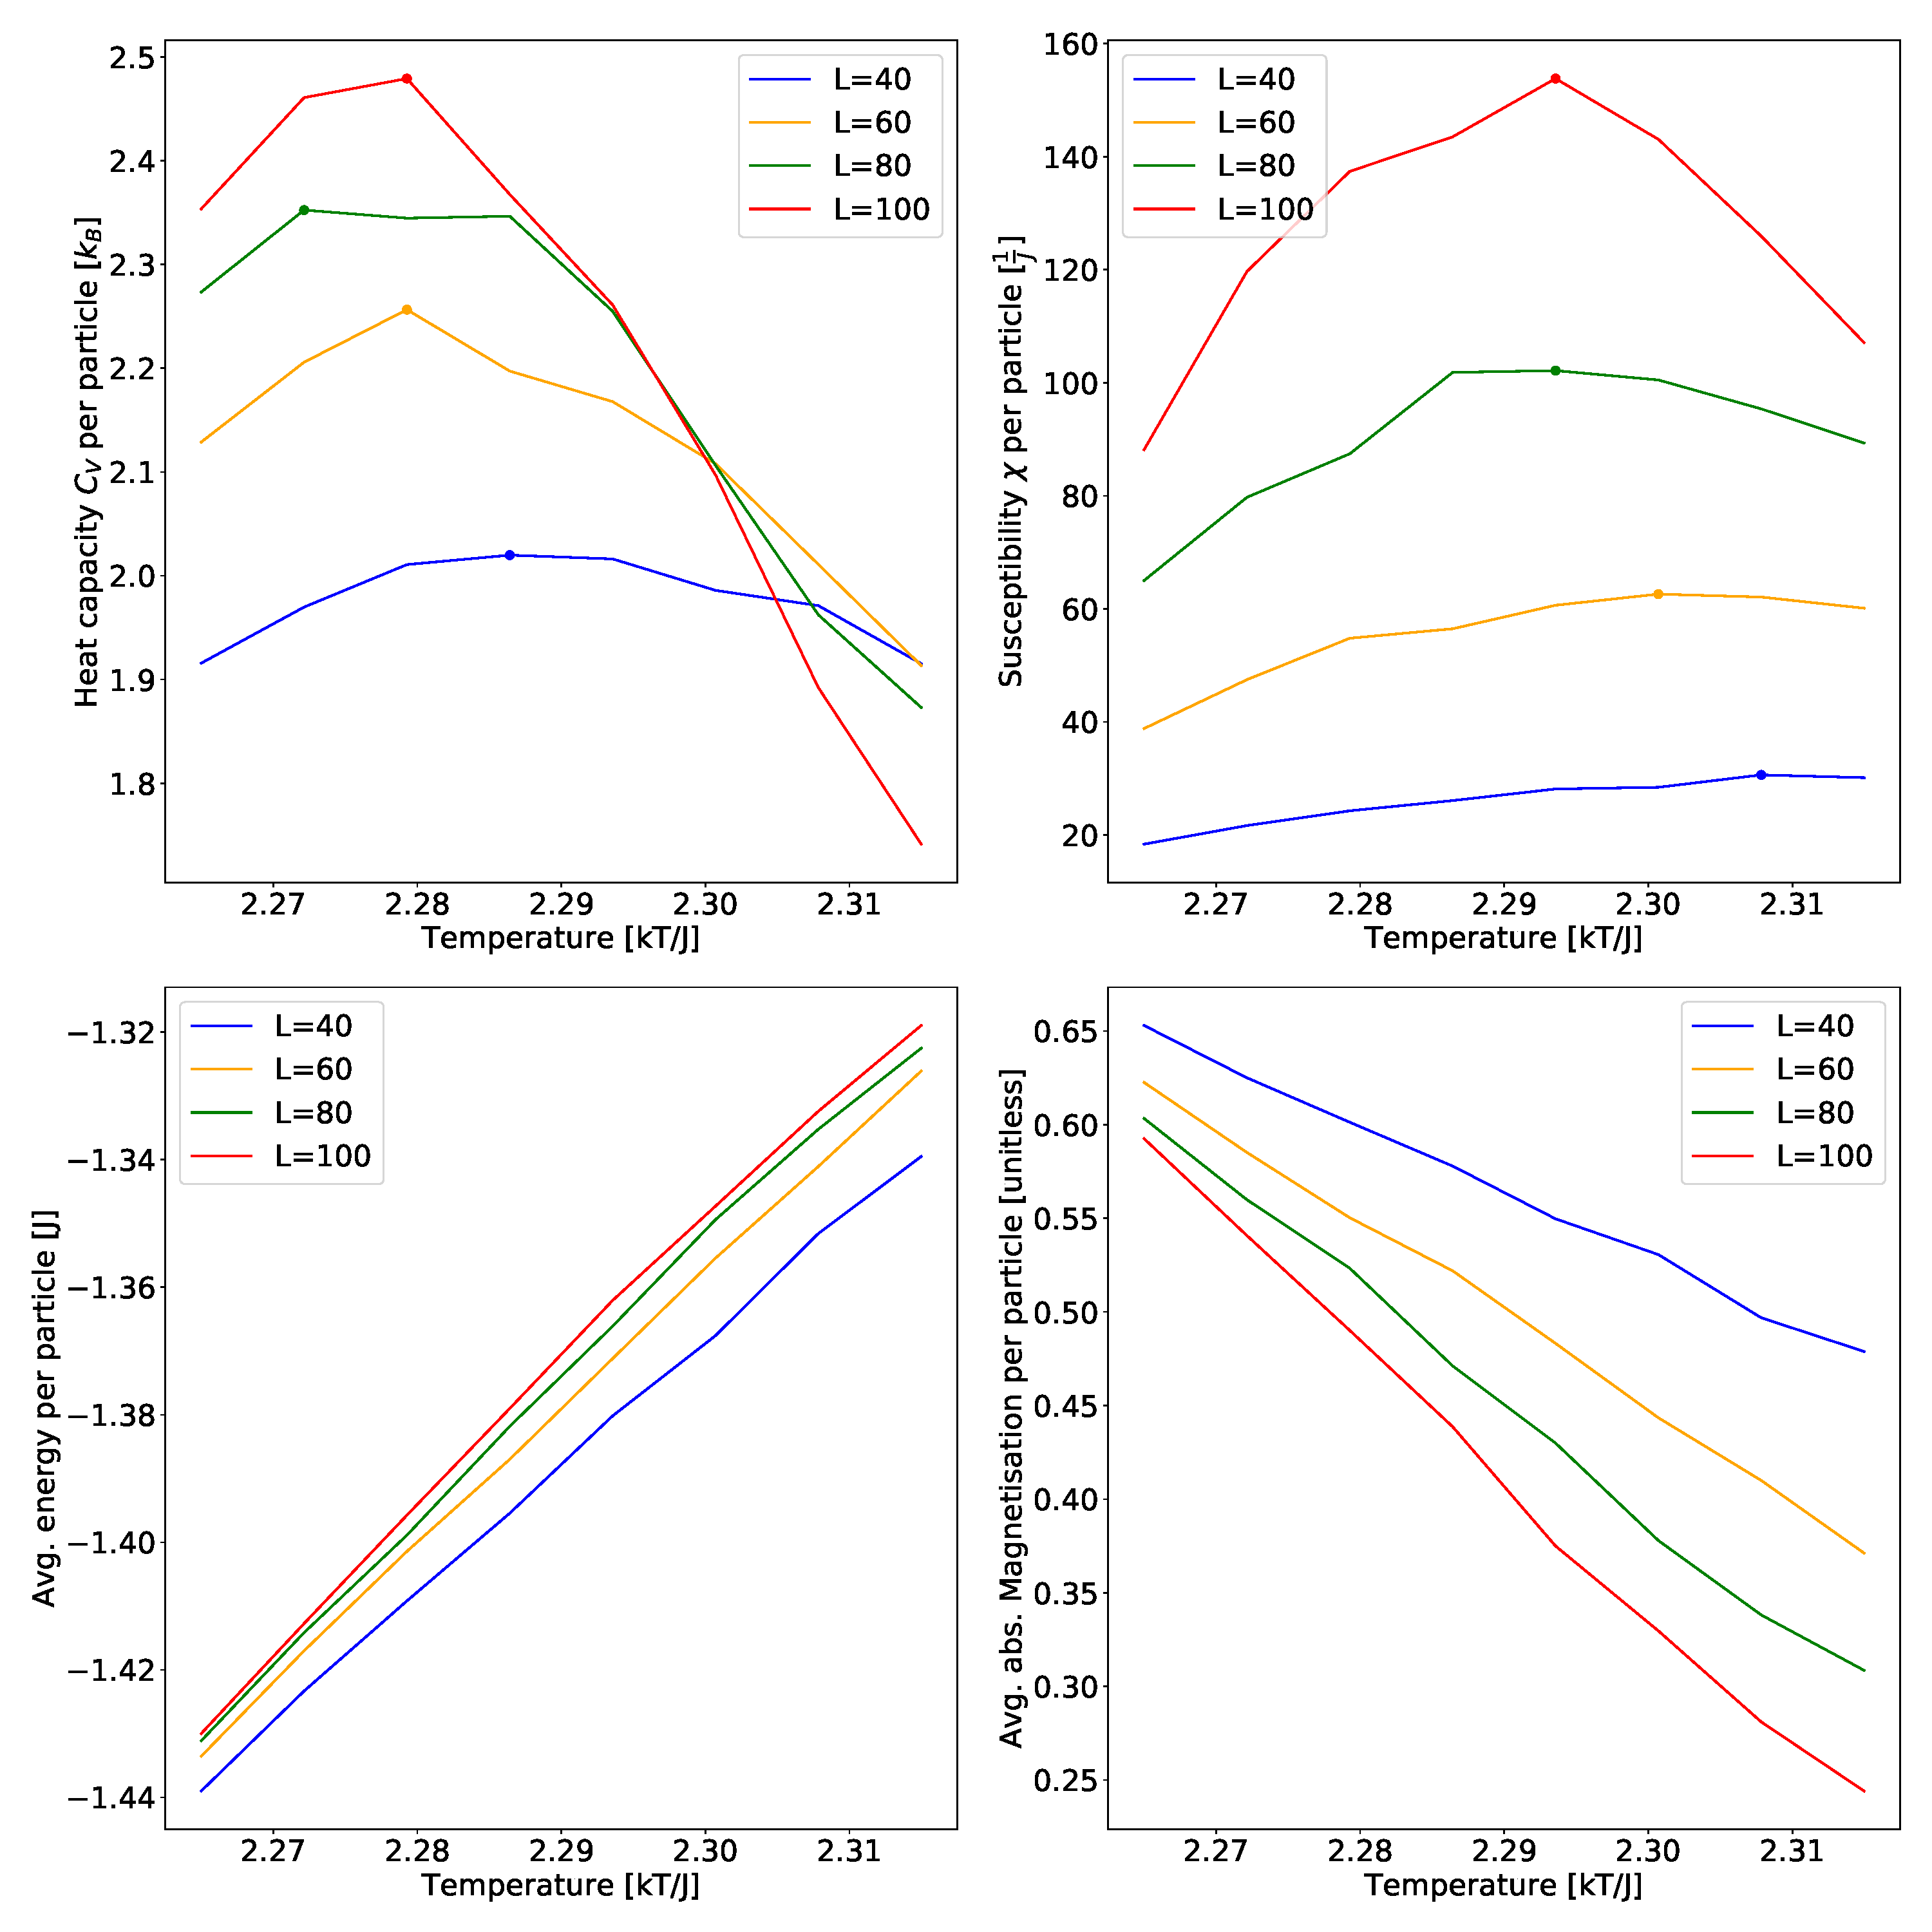
\includegraphics[width=\textwidth]{results_calculations_much_more_accurate.pdf}
\caption[$C_V,\chi,E, |M|$ for T between 2.265 and 2.315]{$C_V,\chi,E$ and $|M|$ as functions of T for  L $ \in \{40,60,80,100\}$ for T between  2.265 and 2.315 with a step length of XXX. For each temperature, XXX simulation steps were carried out. Maximum value is marked for $\chi,C_V$.}\label{for T between 2.265 and 2.315}
\end{figure}
\subsection{Tables}

\begin{table}[H]
\centering
\caption[2x2 lattice rel. errors with  $10^7$ simulation steps]{The largest relative error, at which temperature showed up, and where it showed up for $10^7$ simulation steps in a 2x2 lattice. Temperatures were run in $[2.0,3.0)$ with a uniform spacing of 0.1.}
\begin{tabular}{|r|r|r|}
\hline
Relative error & Temperature & Physical quantity \\ \hline
0.00169        & 2.0         & Heat Capacity     \\ \hline
0.00286        & 2.1         & Heat Capacity     \\ \hline
0.00180        & 2.1         & Heat Capacity     \\ \hline
0.00156        & 2.0         & Heat Capacity     \\ \hline
0.000819       & 2.6         & Heat Capacity     \\ \hline
\end{tabular}
\end{table}
\begin{table}[H]
\centering
\caption[2x2 lattice rel. errors with  $10^6$ simulation steps]{The largest relative error, at which temperature showed up, and where it showed up for $10^6$ simulation steps in a 2x2 lattice. Temperatures were run in $[2.0,3.0)$ with a uniform spacing of 0.1.}
\begin{tabular}{|r|r|r|}
\hline
Relative error & Temperature & Physical quantity \\ \hline
0.00598     & 2.1         & Heat Capacity     \\ \hline
0.00356        & 2.0        & Heat Capacity     \\ \hline
0.00882        & 2.0        & Heat Capacity     \\ \hline
0.00823        & 2.1        & Heat Capacity     \\ \hline
0.00282       & 2.9         & Heat Capacity     \\ \hline
\end{tabular}
\end{table}
\subsection{List of programs}
All programs can be found on \url{https://github.com/adrian2208/FYS3150_collab} in the folder "Project4".


\begin{itemize}
\item[1.] b.cpp - Program with several options of writing to file, different matrices etc., for a given temperature and lattice size
\item[2.] e\_not\_parallel.cpp - Like b, but can run over several lattices and temperatures, more efficient
\item[3.] e.cpp - Same as above, but parallelized with openMPI
\item[4.] vecop.hpp - Several functions
\item[5.] vecop.cpp - Functions, out of which some are used.
\item[6.] tests\_main.cpp - Unit testing.
\item[7.] a.py - Analytical solution. Not properly up to date!
\item[8.] plot\_cv.py - Creates 2x2 plot for the larger simulations, also calculates $T_C(L=\infty)$
\item[9.] plot\_distribution.py Plots the distribution histograms at different temperatures.
\item[10.] plot\_energy\_simulation\_step.py Plots the  avg. energy, the avg. magnetisation and the amount of accepted steps as a function of simulation step.
\item[11.] functions.hpp \& functions.cpp - Contains functions for parallelization, and all the integrands, and some more.
\end{itemize}
\cite{Lecture_Notes_Fall_2015}
\cite{Problem_set_3}
\bibliographystyle{Plain}



\bibliography{citations}



\begin{comment}

$$
\begin{bmatrix}
0 & 0 & 0 & 0 \\
0 & 0 & 0 & 0 \\
0 & 0 & 0 & 0 \\
0 & 0 & 0 & 0 \\
\end{bmatrix}
$$

\begin{lstlisting}[caption=insert caption]
for (unsigned int i = 0; i<100;i++{
}
\end{lstlisting}

\begin{figure}[h]
\includegraphics[width=8cm]{}
\caption{include caption}
\end{figure}

\end{comment}

\end{document}